\chapter{Cloud storage}
After going through CPU and network virtualization, it's time to talk about
proper ways of handling storaged data. In the age of \emph{cloud computing}
there's a huge amount of data to store, access and secure, so novel approches
to system design are necessary. To achieve the goal of cloud computation,
effective data replication and appropriate storage management strategies are
critical.

In the past, storage system were desing according to a
\emph{performance-at-any-cost} philosophy, but now there's been a shift towards
\emph{reliability-at-the-lowest-possible-cost}. For example, data replication
allows concurrent access to data from multiple processors and decreases the
chances of data loss, but maintaining consistency among multiple copies of data
records increases the data management software complexity and could negatively
affect the storage system performance if data is frequently updated.

So, in this chapter we're going to explain some modern strategies adopted
to manage cloud storage while also respecting performance and realibility
requirements.

\section{Preliminary definitions}
Before proceding, we need to fix some concepts.

\begin{definition}[Storage model]
    A storage model describes the layout of a data structure in a physical storage.
\end{definition}
\begin{definition}[Data model]
    A data model captures the most important logical aspects of a data structure
    in a database
\end{definition}

\begin{definition}[Read-write coherence]
    The result of reading of a memory cell, should be the same as the most recent
    writing done on that cell.
\end{definition}
\begin{definition}[Before-or-after atomicity]
    The result of every read or write operation is the same as if that
    operation has been performed completely before or after another read or
    write operation.
\end{definition}

\noindent
\emph{Read-write coherenct} and \emph{Before-or-after atomicity} are two highly
desirable properties of any \emph{storage model}.

\subsection{Types of storage}
There are three main types of storage:
\begin{enumerate}
    \item \emph{Block storage}: data is managed as blocks within sectors and
    tracks. Can be used when storage has access to raw and unformatted hardware
    and is usedfull when both speed and efficiency are important;
    \item \emph{File storage}: data is organized as structured files which are
    managed through a file system. However, this doesn't work very well with
    large amounts of data or high-demands for a particular piece of data;
    \item \emph{Object storage}: data is managed as objects. Typically, each
    object has a gloabal unique identifier and holds both the data itself and
    some metadata. It's possible to access whole objects or blobs of data, but
    random access to data within an object is more difficult;
\end{enumerate}

\noindent
\emph{Block storage} is often used for database because it's the ideal way of
storing relational information. On the other hand, \emph{Object storage} isn't
suitable for databases, but is preferable to store content that can grow without
bounds, for example, backups and archives. Finally, the \emph{File storage} model
can be easily used to create \emph{distributed file system} vian network protocols.

Examples of \emph{Block storage}, \emph{File storage} and \emph{Object storage}
are, respectivelly, Cinder, Google file system and OpenStack Swift.

\section{Block storage}
We'll give a quick look to this model by scratching the surface of \emph{OpenStack
Cinder}. \emph{OpenStack Cinder} implements services and libraries to provide
on-demand, self-service access to block storage resources. It provides API to
interact with storage backends which is also exposed to the cloud. End users can
manage their storage without knowing how it's organized and for both physical and
virtual environments.

\begin{figure}[h!]
    \centering
    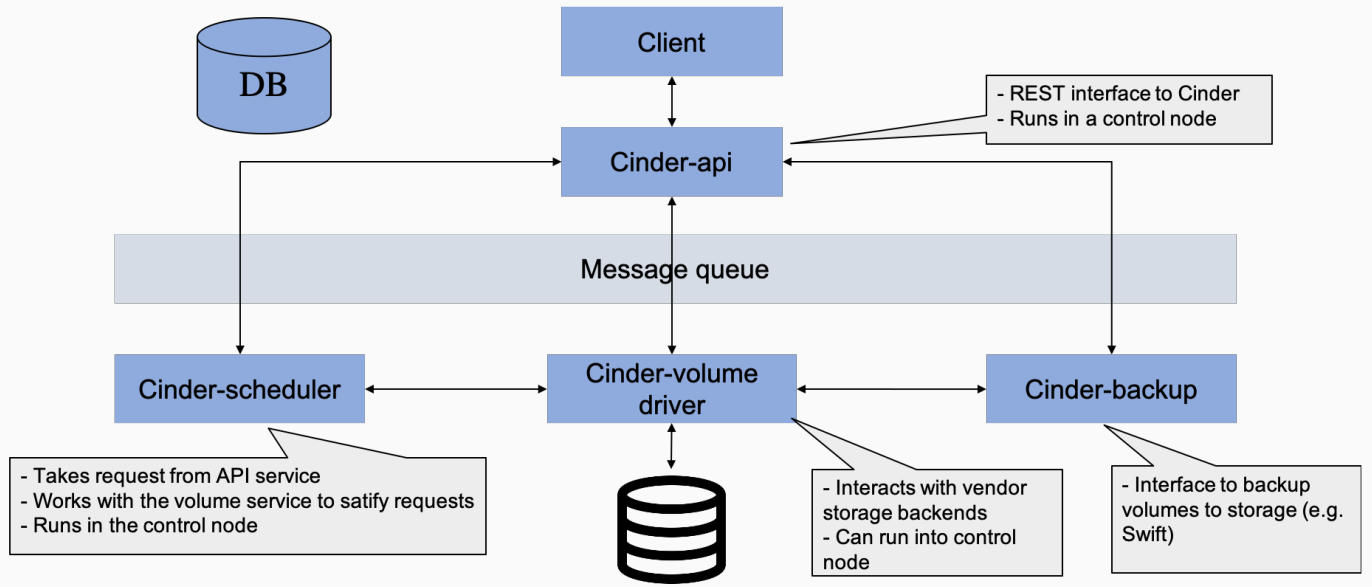
\includegraphics[width=0.7\textwidth]{images/block-model-cinder.png}
    \caption{\emph{OpenStack Cinder basic architecture}}
\end{figure}

\noindent
\emph{Cinder} APIs allow users to create and delete volumes and snaphots (for
backup pourposes). Attach or detach volumes for the available storage, clone and
extend them, and so on.

\section{Distributed file system}
Again, we'll start by giving some definitions.

\begin{definition}[File]
    A file is a linear array of cells stored on a persistent storage device. It
    is seen by application as a collection of logical records, and it's stored
    on a physical device as a set of physical records, or blocks, of size
    dictated by the physical media.
\end{definition}
\begin{definition}[File pointer]
    A file pointer is a cell used as starting point for a read or write operation.
\end{definition}

\noindent
A file has a logical organisation reflects the data model from the perspective of
the application, and a physical orgnisation that reflects the storage model and
describes the manner the file is stored on a given storage media.

\begin{definition}[File system]
    A file system is a collection of directories and each directory provides
    information about a set of files. A file system controls how data is stored
    and retrieved.
\end{definition}

\subsection{Unix File System}
The \emph{Unix File System} (\emph{UFS}) has both a layered and hierarchical
design. The first allows it to separate the physical file structure from the
logical one, and this becomes usefull when dealing with files stored both locally
and remotely. The hierarchical design, on the other hand, allows grouping of
files directories, supports multiple levels of directories and collections of
directories and files; thus, supporting a good degree of scalability.

The metadata that \emph{UFS} uses includes file owner, access rights, creation
time, time of the last modification, file size, the structure of the file and
the persistent storage device cells where data is stored. All of these are
memorized in a structure called \emph{inode}. Each \emph{inode} holds information
about individual files and directories and is kept on persistent media together
with the actual data.

\bigskip\noindent
Going back to \emph{UFS} layering, there are two layers:
\begin{itemize}
    \item \emph{Lower layer}: is about the physical organisation and is furderly
    separated into three sub-layers:
    \begin{itemize}
        \item \emph{Block layer}: responsible for locating individual blocks on
        the physical device;
        \item \emph{File layer}: reflects the organisation of blocks into files;
        \item \emph{Inode layer}: provides metadata for files and directories;
    \end{itemize}
    \item \emph{Upper layer}: is about the logical orgnisation;
\end{itemize}

\newpage
\begin{figure}[ht!]
    \centering
    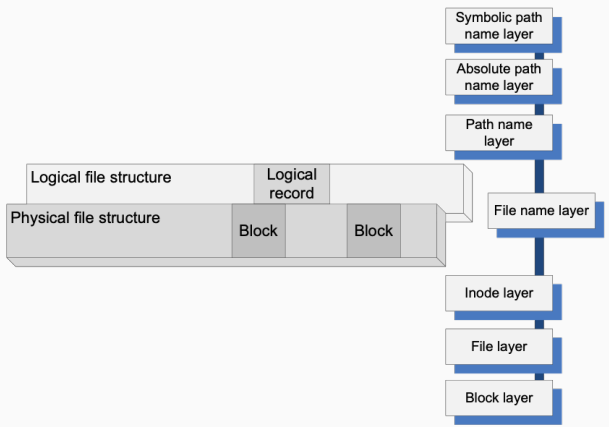
\includegraphics[width=0.6\textwidth]{images/ufs-layering.png}
    \caption{\emph{UFS} layering}
\end{figure}

\subsection{Network File System}
The \emph{Network File System} (\emph{NFS}) is designed to provide the same
semantics as the \emph{UFS} to ensure compatiblity with existing applications.
\emph{NFS} is based on the client-server paradigm and, in particular, clients
runs on the local host and interact with the server via remote procedure calls.

Each remote file is identified by a 32-bit file handler rather than a file
descriptor like in \emph{UFS}. A file handler is obtained combining a file
system identication, an \emph{inode} number and a generation number.

\begin{figure}[h!]
    \centering
    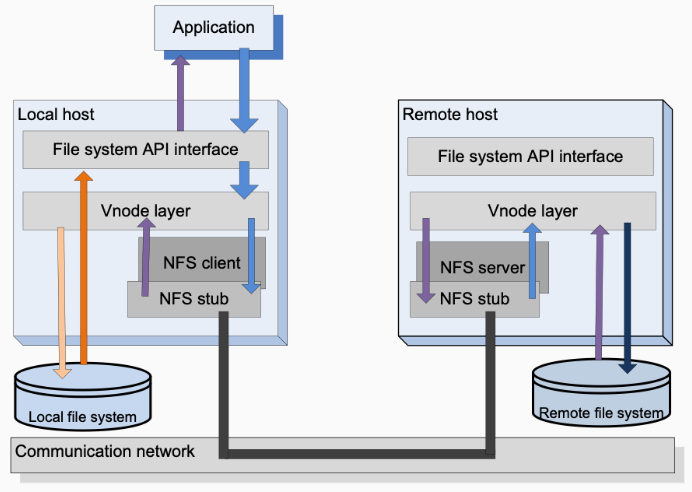
\includegraphics[width=0.6\textwidth]{images/nfs-design.png}
    \caption{\emph{NFS} design}
\end{figure}

\noindent
As the image shows, instead of an \emph{inode layer} the \emph{NFS} has a
\emph{vnode layer} which implements file operation in a uniform manner,
regardless of whether the file is local or remote. Also, an operation targeting
a local file is directed to the local file system without involving the \emph{NFS}.

When a client interacts with the server, the client-side \emph{NFS} packages the
relevant information about target, then sends those packeged information to the
server-side \emph{NFS}. The latter then passes the received information to the
\emph{vnode layer} of the remote host which finally directs it to the remote
file system.

\newpage
\begin{table}[ht!]
    \centering
    \begin{tabular}{|l|l|c|l|p{0.5\textwidth}|}
        \hline
        \textbf{API} & \textbf{Description} && \textbf{API} & \textbf{Description}\\
        \hline
        \texttt{fd} & File descriptor && \texttt{dfh} & The directory when the file
        handle can be found\\
        \hline
        \texttt{fh} & File handle && \texttt{count} & Number of bytes to be transferred\\
        \hline
        \texttt{fname} & File name && \texttt{buf} & Buffer used to transfer data\\
        \hline
        \texttt{dname} & Directory name && \texttt{device} & The device in which the
        file system is located\\
        \hline
    \end{tabular}
    \caption{\emph{NFS} APIs}
\end{table}

\begin{figure}[h!]
    \centering
    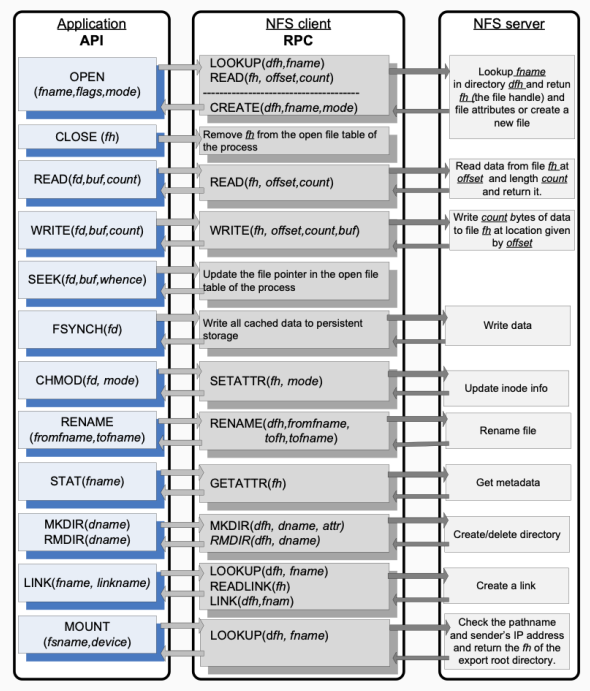
\includegraphics[width=0.6\textwidth]{images/nfs-remote-calls.png}
    \caption{\emph{UFS} APIs and corresponding \emph{NFS} remote procedure calls}
\end{figure}

\paragraph{Common design choices for distributed file system}
The vast majority of distributed file systems has been implemented in similar
ways. That's not so surprising if we think that they all need to solve the same
problems and that the possible or best solutions to choose from are limited.

Tipically every distributed file system is implented in a way that once a file
is closed, the server will have the newest version of it on persisten storage.
Another concern is about what to do when writing on a file. The possible
solutions are two:
\begin{enumerate}
    \item \emph{Write-through}: block is written to the disk as soon as it is
    available on the cache. This approch increases reliability, but takes more
    time to complete each write operation;
    \item \emph{Delay in write-back}: a block is first written to cache and
    writing on the disk is delayed for a time in the order of tens of seconds.
    This speeds up writings and avoids useless writing when data is discarded
    before the time to save it to the disk. However, data can be lost in case
    of system failures;
\end{enumerate}

\noindent
Finally, how should the system act when multiple clients tries to access the
same file at the same time. The approches are two:
\begin{enumerate}
    \item \emph{Sequential write-sharing}: a file cannot be opened simultaneously
    for reading and writing by several clients;
    \item \emph{Concurrent write-sharing}: multiple clients can modify the file
    at the same time;
\end{enumerate}

\subsection{General Parallel File System}
